\documentclass[11pt]{article}
\title{Machine Learning Homework 03 – Report}
\author{Adam Catto}
\date{ }
\usepackage{graphicx}
\usepackage{amsmath}
%\usepackage{mathscr}

\usepackage{amsmath}
\newcommand{\y}{\mathbf{y}}
\begin{document}
\maketitle
\section{Solution}
The goal of this assignment was to implement multiclass logistic regression (i.e. softmax regression), train it on the sklearn digits dataset, and test its accuracy. There was some preprocessing to be done, namely to compute concrete features from the raw data and transform them. I computed three concrete features –– x-symmetry, y-symmetry, and density. The methods for computing these features were:
\begin{itemize}
	\item{\textbf{x-symmetry}} flip the image matrix from left-to-right, compute the element-wise differences, normalize these values, and return the magnitude of the corresponding vector (gotten by flattening the new image matrix)
	
	\item{\textbf{y-symmetry}} flip the image matrix from up-to-down, compute the element-wise differences, normalize these values, and return the magnitude of the corresponding vector (gotten by flattening the new image matrix)
	
	\item{\textbf{density}} this is simply the average of all pixel intensities in the image. Add them up and divide by 64.
\end{itemize}

This is a dimensionality reduction technique; we reduce the number of features from 64 to 3. However, these features alone may not be informative enough, so we apply a transformation to the feature space; the chosen transformation was to fit the features to a cubic polynomial. The resulting feature space is 20-dimensional. I also ran the experiments on the raw data, to test how well the transformation worked towards classification accuracy.  \\
 \\
To classify the images, I implemented a multiclass logistic regression function with regularization; the chosen technique was softmax regression (as opposed to one-vs-all classification), with cross-entropy loss function. The softmax function is computed as 
$$ \frac{exp(x}{\sum_i exp(x_i} $$
This is done to create a probability distribution from the computed data; this is useful for weight-updating, to be discussed later.\\
 \\
 Using the softmax function, we compute the cross-entropy loss as 
$$ \frac{1}{n}\sum_n (\ln softmax(x\cdot w) \cdot y) $$

where $x$ is the data matrix, $w$ is the weight matrix, and $y$ is the set of target variables. The gradient of the loss function is computed to be 
$$ \nabla\mathcal{L} = x^T \times (softmax(x\cdot w) - y) $$ 
normalized by its magnitude, $|| \nabla\mathcal{L}||$\\
 \\
The training of the classifier went as follows: over the course of a specified number of iterations  (in this case, 500), multiply the training data matrix by the weights and compute the softmax of each row – this gives the softmax distribution for the row. The key here is that the larger a particular value is in the distribution, the more strongly the classifier associates that sample with the class at the value's index. When doing prediction, we take the argmax over the softmax distribution as our prediction, but for training we simply are trying to update the weights maximally in the proper direction – the direction opposite of the gradient of the loss function. The main idea behind this step is: take the row-wise differences between the softmax output and the actual (one-hot-encoded) target variables, which is multiplied on the left by the transpose of the training data, and then normalized by its magnitude. The weights are then updated against this direction, parametrized by (1) a learning rate (how far along the direction we move) and (2) a regularization (Lagrangian) term – in this case, the inverse of the square of the magnitude of the weights, itself parametrized by some constant between zero and one.\\
  \\
In the prediction stage, we take the weights at the end of the training stage, and use these in the computation of the softmax output; from the softmax output, take the argmax (as mentioned in the preceding paragraph), and use this as the predicted value. The accuracy score is computed as $\frac{\# correct}{\# total}$.

\section{Results}
I ran experiments on data from the digits dataset. The original dataset contains 1797 samples and 64 features. As a dimensionality reduction technique, I computed three features from the data (as mentioned in the previous section: x-symmetry, y-symmetry, density) and used a cubic polynomial transform on these features to map them into a 20-dimensional feature space. I compared the accuracy of the classifier on the original dataset as well as the transformed dataset, using a learning rate of 0.1, 500 iterations, and varied regularization factors of 0, 0.1, 0.01, and 0.001. Additionally, the accuracy was evaluated using five-fold cross-validation – that is, partition the train-test-splits five ways, and take the average of the accuracies across those 5 splits. The training stage was vectorized, so the weight-updating in each epoch was done in parallel, rather than looped row-by-row.\\
 \\
 The classifier performed much better on the non-transformed dataset, and similarly across regularization terms. 
 
When using regularization, a regularization factor of 0.01 appeared to be best for both datasets.\\
 \\
 $
 \begin{bmatrix}
 	\text{Regularization Factor} & \text{Transform Accuracy} & \text{Non-Transform-Accuracy}\\
 	0 & 0.333 & 0.910 \\
 	0.1 & 0.329 & 0.910\\
 	0.01 & 0.331 & 0.912\\
 	0.001 & 0.328 & 0.907
 \end{bmatrix}
 $\\
 \\
Although the difference was insignificant. Plots for the losses per iteration for each of the regularization terms (left-to-right: 0, 0.1, 0.01, 0.001) for one fold are (for transformed data):\\
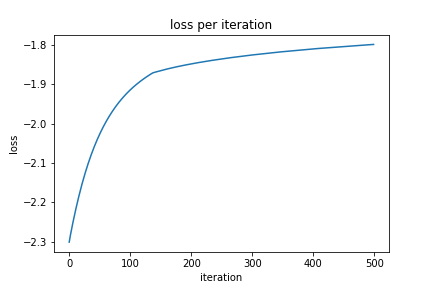
\includegraphics[scale=0.2]{images/loss_transform_0000}
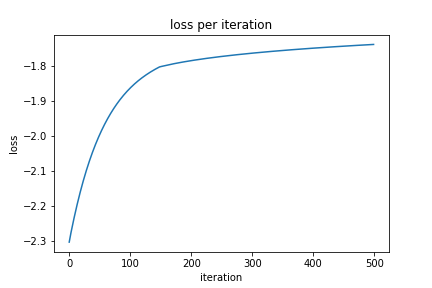
\includegraphics[scale=0.2]{images/loss_transform_0001}
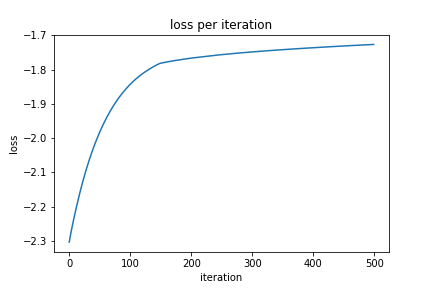
\includegraphics[scale=0.2]{images/loss_transform_0002}
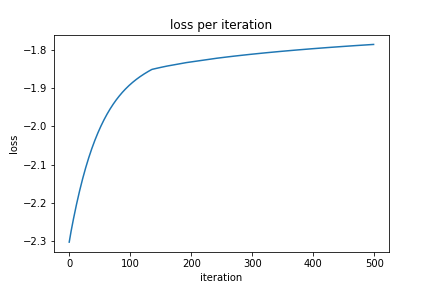
\includegraphics[scale=0.2]{images/loss_transform_0003}\\
 \\
and for the raw data:\\
 \\
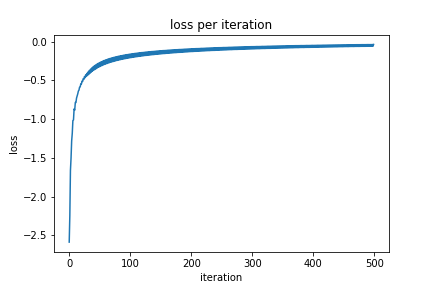
\includegraphics[scale=0.2]{images/loss_no_transform_0000}
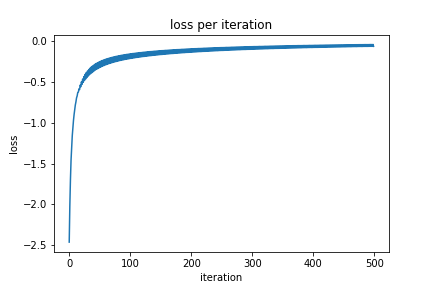
\includegraphics[scale=0.2]{images/loss_no_transform_0001}
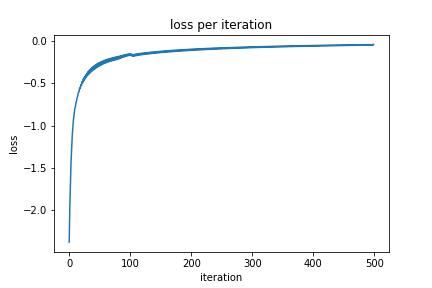
\includegraphics[scale=0.2]{images/loss_no_transform_0002}
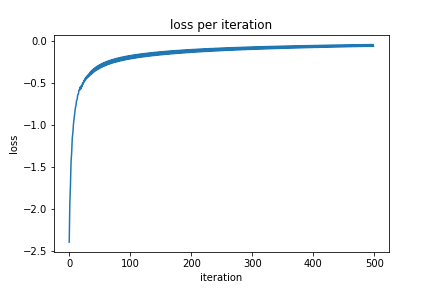
\includegraphics[scale=0.2]{images/loss_no_transform_0003}\\
 \\
 This suggests that the transformation, while reducing dimensionality, did not seem to capture features that distinguished the classes well enough. The fact that the loss function did not converge around zero (and seemed to be converging around -1.5) suggests that it is not an issue of training more, but instead it is an issue of improper feature engineering. This suggests that either the cubic transformation is not an appropriate model, or (more likely) the concrete features computed were similar enough across classes that the separability of data by class was low. This is not necessarily an issue of finding the appropriate transformation – it is more an issue of computing relevant features that properly separate the classes.
\end{document}